\subsection{K-微分的函子性质}

命题19。设

\[
\begin{array}{c c c} \mathrm{K} & \xrightarrow {\rho} & \mathrm{K} ^ {\prime} \\ \Big \downarrow_ {\eta} & & \Big \downarrow_ {\eta^ {\prime}} \\ \mathrm{A} & \xrightarrow {u} & \mathrm{A} ^ {\prime} \end{array}
\]

是交换环同态的交换图， \(\eta\) （相应地 \(\eta'\) ) 使得

A（相应地，A'）成为 K-代数（相应地，K'-代数）。存在且仅存在一个 A-线性映射 \(v: \Omega_{\mathbf{K}}(\mathbf{A}) \to \Omega_{\mathbf{K}'}(\mathbf{A}')\) 使该图表交换

\pandocbounded{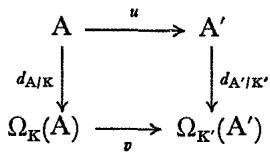
\includegraphics[keepaspectratio]{images/part004_9ff9737d.jpg}}

\(d_{\mathbf{A}^{\prime} / \mathbf{K}^{\prime}}\circ u\) 是 A 的、取值于 A-模 \(\Omega_{\mathbf{K}^{\prime}}(\mathbf{A}^{\prime})\) 的一个 K-导子； \(v\) 的存在性与唯一性随后由第11号命题18得出。

命题19中的映射 v 将记作 \(\Omega(u)\) ；若存在一个由交换环同态构成的交换图

\pandocbounded{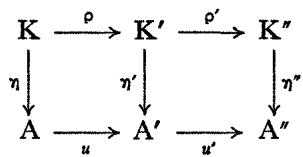
\includegraphics[keepaspectratio]{images/part004_26fbb1e8.jpg}}

由命题19的唯一性性质，立即得出

\[
\Omega (u ^ {\prime} \circ u) = \Omega (u ^ {\prime}) \circ \Omega (u).
\]

由于 \(\Omega_{\mathbf{K}'}(\mathbf{A}')\) 是一个 \(\mathbf{A}'\) -模，由 \(\Omega(u)\) 我们典范地导出一个 \(\mathbf{A}'\) -线性映射

\[
\Omega_ {0} (u): \Omega_ {\mathbf {K}} (\mathrm{A}) \otimes_ {\mathrm{A}} \mathrm{A} ^ {\prime} \rightarrow \Omega_ {\mathbf {K} ^ {\prime}} (\mathrm{A} ^ {\prime})\tag{41}
\]

，使得 \(\Omega(u)\) 是 \(\Omega_0(u)\) 与典范同态 \(i_{\mathbf{A}}: \Omega_{\mathbf{K}}(\mathbf{A}) \to \Omega_{\mathbf{K}}(\mathbf{A}) \otimes_{\mathbf{A}} \mathbf{A}'\) 的复合。对每个 \(\mathbf{A}'\) -模 \(\mathbf{E}'\) ，有一个交换图

\pandocbounded{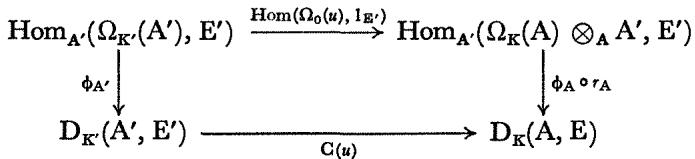
\includegraphics[keepaspectratio]{images/part004_95f64194.jpg}}

（其中 \(\mathbf{C}(u)\) 是映射 \(D \mapsto D \circ u\) （第7号，命题9），而 \(r_{A}\) 是典范同构

\[
\operatorname{Hom} \left(i _ {\mathrm{A}}, 1 _ {\mathrm{E} ^ {\prime}}\right): \operatorname{Hom} _ {\mathrm{A} ^ {\prime}} \left(\Omega_ {\mathrm{K}} (\mathrm{A}) \otimes_ {\mathrm{A}} \mathrm{A} ^ {\prime}, \mathrm{E} ^ {\prime}\right)\rightarrow \operatorname{Hom} _ {\mathrm{A}} \left(\Omega_ {\mathrm{K}} (\mathrm{A}), \mathrm{E} ^ {\prime}\right);
\]

这直接由命题19以及同构 \(\phi_{\mathbf{A}}\) 和 \(\phi_{\mathbf{A}^{\prime}}\) 的定义得出。

命题20. 假设 \(\mathbf{A}' = \mathbf{A} \otimes_{\mathbb{K}} \mathbf{K}'\) ，其中 \(\eta': \mathbf{K}' \to \mathbf{A}'\) 和 \(u: \mathbf{A} \to \mathbf{A}'\) 是典范同态。则 \(\mathbf{A}'\) -线性映射

\[
\Omega_ {0} (u): \Omega_ {\mathbf {K}} (\mathrm{A}) \otimes_ {\mathbf {A}} \mathrm{A} ^ {\prime} \rightarrow \Omega_ {\mathbf {K} ^ {\prime}} (\mathrm{A} ^ {\prime})
\]

是一个同构。

由于图(42)中竖直箭头是双射，问题归结为证明：对每个A'-模E'，图(42)中的同态C(u):D → D ∘ u是双射（II，§2，第1号，定理1）。现在Hom(u, 1\_E') : Hom\_K'(A ⊗\_K K', E') → Hom\_K(A, E')是同构（II，§5，第1号，命题1），而C(u)是它在D\_K'(A', E')上的限制，因此是单射；此外，若 f: A' → E' 是一个 K'-线性映射，使得

\[
f \circ u: \mathrm{A} \rightarrow \mathrm{E} ^ {\prime}
\]

是 K-导子，则由 \(f\) 是 \(\mathbf{K}'\) -线性的以及 \(f((x \otimes 1)(y \otimes 1)) = (y \otimes 1)f(x \otimes 1) + (x \otimes 1)f(y \otimes 1)\) （对 A 中的 \(x, y\) ）这一事实，立即得出 \(f\) 是一个 \(\mathbf{K}'\) -导子，因为元素 \(x \otimes 1\) （对 \(x \in A\) ）构成 \(\mathbf{K}'\) -模 \(A'\) 的一个生成系；这就完成了 \(C(u)\) 是双射的证明。

从现在起，我们把注意力限制在 \(\rho: \mathbf{K} \to \mathbf{K}'\) 是 \(\mathbf{K}\) 的恒等映射的情形；每个 K-代数同态 \(u: \mathbf{A} \to \mathbf{B}\) 因此被映为一个 B-线性映射

\[
\Omega_ {0} (u): \Omega_ {\mathbf {K}} (\mathrm{A}) \otimes_ {\mathbf {K}} \mathrm{B} \rightarrow \Omega_ {\mathbf {K}} (\mathrm{B}).\tag{43}
\]

另一方面，我们可以考虑 A-微分的 B-模 \(\Omega_{\mathbf{A}}(\mathbf{B})\) ，因为 B 通过 u 成为 A-代数；典范导子 \(d_{\mathrm{B/A}}: \mathbf{B} \to \Omega_{\mathbf{A}}(\mathbf{B})\) 当然更是 K-导子，因此它唯一地分解为

\[
\mathbf {B} \xrightarrow {d _ {\mathbf {B} / \mathbf {K}}} \Omega_ {\mathbf {K}} (\mathbf {B}) \xrightarrow {\Omega_ {u}} \Omega_ {\mathbf {A}} (\mathbf {B})
\]

其中 \(\Omega_{u}\) 是 B-线性映射（第11号，命题18）。对每个 B-模 E，有交换图

\[
\begin{array}{c} \operatorname{Hom} _ {\mathbf {B}} (\Omega_ {\mathbf {A}} (\mathbf {B}), \mathrm{E}) \xrightarrow {\operatorname{Hom} (\Omega_ {u} , 1 _ {\mathbf {E}})} \operatorname{Hom} _ {\mathbf {B}} (\Omega_ {\mathbf {K}} (\mathbf {B}), \mathrm{E}) \\ \phi_ {\mathbf {A}, \mathbf {B}} \Biggl \downarrow \\ \mathrm{D} _ {\mathbf {A}} (\mathrm{B}, \mathrm{E}) \xrightarrow [ j _ {u} ]{} \mathrm{D} _ {\mathbf {K}} (\mathrm{B}, \mathrm{E}) \end{array}\tag{44}
\]

其中 \(j_{u}\) 是典范单射（第7号）；这直接由第11号的命题18得出。

命题21：B-线性映射的序列

\[
\Omega_ {\mathbf {K}} (\mathrm{A}) \otimes_ {\mathbf {A}} \mathrm{B} \xrightarrow {\Omega_ {0} (u)} \Omega_ {\mathbf {K}} (\mathrm{B}) \xrightarrow {\Omega_ {u}} \Omega_ {\mathbf {A}} (\mathrm{B}) \to 0\tag{45}
\]

是正合的。

只需验证：对每个B-模E，序列

\[
\begin{array}{c} 0 \to \operatorname{Hom} _ {\mathrm{B}} (\Omega_ {\mathrm{A}} (\mathrm{B}), \mathrm{E}) \xrightarrow {\operatorname{Hom} (\Omega_ {\mathrm{u}} , 1 _ {\mathrm{E}})} \operatorname{Hom} _ {\mathrm{B}} (\Omega_ {\mathrm{K}} (\mathrm{B}), \mathrm{E}) \\ \xrightarrow {\operatorname{Hom} (\Omega_ {0} (u) , 1 _ {\mathrm{E}})} \operatorname{Hom} _ {\mathrm{B}} (\Omega_ {\mathrm{K}} (\mathrm{A}) \otimes_ {\mathrm{A}} \mathrm{B}, \mathrm{E}) \end{array}
\]

是正合的（II，§2，第1号，定理1）；但由于在交换图（42）和（44）中垂直箭头是同构的，只需证明序列

\[
0 \longrightarrow \mathrm{D} _ {\mathrm{A}} (\mathrm{B}, \mathrm{E}) \xrightarrow {j _ {u}} \mathrm{D} _ {\mathrm{K}} (\mathrm{B}, \mathrm{E}) \xrightarrow {\mathrm{C} (u)} \mathrm{D} _ {\mathrm{K}} (\mathrm{A}, \mathrm{E})
\]

是正合的，这正是第7号的命题11。

现在我们考虑 K-代数同态 \(u: \mathbf{A} \to \mathbf{B}\) 是满射的情形；若 \(\mathfrak{J}\) 是其核，则 \(\mathbf{B}\) 同构于 \(\mathbf{A} / \mathfrak{J}\) 。我们考虑典范导子的限制 \(d| \mathfrak{J}: \mathfrak{J} \to \Omega_{\mathbf{K}}(\mathbf{A})\) （其中 \(d = d_{\mathbf{A} / \mathbf{K}}\) ）以及复合 A-线性映射

\[
d ^ {\prime}: \mathfrak {J} \xrightarrow {d | \mathfrak {J}} \Omega_ {\mathrm{K}} (\mathrm{A}) \xrightarrow {i _ {\mathrm{A}}} \Omega_ {\mathrm{K}} (\mathrm{A}) \otimes_ {\mathrm{A}} \mathrm{B}.
\]

那么 \(d^{\prime}(\mathfrak{J}^{2}) = 0\) ，因为，对于 \(x, y\) 在 \(\mathfrak{J}\) ,

\[
d ^ {\prime} (x y) = d (x y) \otimes 1 = (x. d y + y. d x) \otimes 1 = d y \otimes u (x) + d x \otimes u (y) = 0
\]

因为 \(u(x) = u(y) = 0\) 。因此我们由 \(d'\) 通过过渡到商得到一个 A-线性映射

\[
\bar {d} \colon \mathfrak {J} / \mathfrak {J} ^ {2} \rightarrow \Omega_ {\mathrm{K}} (\mathrm{A}) \otimes_ {\mathrm{A}} \mathrm{B}
\]

且由于 \(\mathfrak{J}\) 零化 A-模 \(\mathfrak{J} / \mathfrak{J}^2\) ， \(\bar{d}\) 是一个 B-线性映射。

命题 22。设 \(\mathfrak{J}\) 是交换 K-代数 A 的一个理想，B = A/ \(\mathfrak{J}\) ， \(u:A\to B\) 为典范同态。B-线性映射的序列

\[
\mathfrak {J} / \mathfrak {J} ^ {2} \xrightarrow {\overline {{d}}} \Omega_ {\mathrm{K}} (\mathrm{A}) \otimes_ {\mathrm{A}} \mathrm{B} \xrightarrow {\Omega_ {0} (u)} \Omega_ {\mathrm{K}} (\mathrm{B}) \to 0\tag{46}
\]

因而是正合的。

注意， \(\Omega_{\mathbf{K}}(\mathbf{A}) \otimes_{\mathbf{A}} \mathbf{B}\) 与 \(\Omega_{\mathbf{K}}(\mathbf{A}) / \mathfrak{J} \Omega_{\mathbf{K}}(\mathbf{A})\) 相等同，且 \(\bar{d}\) 的像就是 \(d(\mathfrak{J})\) 在这个商模中的像； \(\Omega_{\mathbf{K}}(\mathbf{A}) \otimes_{\mathbf{A}} \mathbf{B}\) 关于 \(\operatorname{Im}(\bar{d})\) 的商因此等同于商 \(\Omega_{\mathbf{K}}(\mathbf{A}) / \mathbf{N}\) ，其中 \(\mathbf{N}\) 是由 \(\mathfrak{J} \Omega_{\mathbf{K}}(\mathbf{A})\) 和 \(d(\mathfrak{J})\) 生成的子 A-模。此外，复合映射

\[
\mathrm{A} \xrightarrow {d _ {\mathrm{A} / \mathrm{K}}} \Omega_ {\mathrm{K}} (\mathrm{A}) \longrightarrow \Omega_ {\mathrm{K}} (\mathrm{A}) / \mathrm{N}
\]

是一个 K-导子（第7号，命题9），并且由于它在 \(\mathfrak{J}\) 上为零（根据 N 的定义），当过渡到商时，它定义了一个 K-导子 \(D_0:B\to \Omega_{\mathbb{K}}(A) / N\) .

考虑到泛映射问题解的唯一性，可以归结为证明：对于每个 B-模 E 和每个 K-导子 D: B → E，存在唯一的 B-线性映射 g： \(\Omega_{\mathrm{K}}(\mathrm{A})/\mathrm{N} \rightarrow \mathrm{E}\) ，使得 \(D = g \circ D_{0}\) 。但是，复合映射 D ∘ u: A → E 是一个 K-导子（第7号，命题9），因此存在且仅存在一个 A-线性映射 f： \(\Omega_{\mathrm{K}}(\mathrm{A}) \rightarrow \mathrm{E}\) ，使得 \(f \circ d_{A/K} = D \circ u\) 。这个关系式已经表明 f 在 \(d(\mathfrak{J})\) 上为零；又因为 E 是 B-模， \(\mathfrak{J} E = \{0\}\) ，所以 f 在 \(\mathfrak{J} \Omega_{\mathrm{K}}(\mathrm{A})\) 上为零；因此 f 在 N 上为零，并在取商后定义了一个 B-线性映射 g： \(\Omega_{\mathrm{K}}(\mathrm{A})/\mathrm{N} \rightarrow \mathrm{E}\) ，使得 \(g \circ D_{0} = D\) ；g 的唯一性由 f 的唯一性得出。

不要以为，即使 \(u: \mathbf{A} \to \mathbf{B}\) 是单射同态， \(\Omega_0(u): \Omega_{\mathbf{K}}(\mathbf{A}) \otimes_{\mathbf{A}} \mathbf{B} \to \Omega_{\mathbf{K}}(\mathbf{B})\) 也是单射（练习5）。然而我们有如下命题：

命题23。设 A 是一个整 K-代数，B 是其分式域，且 \(u: \mathbf{A} \to \mathbf{B}\) 为典范单射。则 \(\Omega_0(u): \Omega_{\mathbf{K}}(\mathbf{A}) \otimes_{\mathbf{A}} \mathbf{B} \to \Omega_{\mathbf{K}}(\mathbf{B})\) 是一个同构。

利用图(42)中竖直箭头是双射这一事实，问题归结为证明：对于B上的每一个向量空间E，映射 \(\mathrm{C}(u):\mathrm{D}_{\mathrm{K}}(\mathrm{B},\mathrm{E})\to\mathrm{D}_{\mathrm{K}}(\mathrm{A},\mathrm{E})\) 是双射。但这可由以下事实推出：A到E的每一个K-导子都能唯一地延拓为B到E的K-导子（第5号，命题5）。

